\hspace{1cm} Jak już wcześniej naznaczyłem posłużę się LMS Moodle. Jedna z zalet tej platformy jest fakt, że Moodle może z powodzeniem być uruchomiony na każdym serwerze, który umożliwia korzystanie z PHP\footnote{PHP~-~Personal~Home~Page, obiektowy, skryptowy język programowania zaprojektowany do generowania stron internetowych w czasie rzeczywistym.} i baz danych. Najlepsze działanie i najwięcej wsparcie ze strony społeczeństwa Moodle ma serwer Apache\footnote{Apache - otwarty serwer HTTP dostępny dla wielu systemów operacyjnych (m.in. UNIX, GNU/Linux, BSD, Mac OS X, Microsoft Windows)} i baz danych MySQL\footnote{MySQL~-~wolnodostępny system zarządzania relacyjnymi bazami danych. MySQL rozwijany jest przez firmę Oracle. Wcześniej przez większość czasu jego tworzeniem zajmowała się szwedzka firma MySQL AB. MySQL AB została kupiona 16 stycznia 2008 roku przez Sun Microsystems, a ten 27 stycznia 2010 roku przez Oracle.}. Te wymagania nie są wygórowane i spełnia je większość komercyjnych serwisów hostingowych, nawet tych najtańszych. Można również znaleźć w sieci darmowe serwisy hostingi umożliwiające poprawne zainstalowanie i funkcjonowanie platformy, np. \href{http://fazz.pl}{Fazz}. \\
\ \\
System zarządzania nauczaniem Moodle'a zajmuje trzy lokalizacje na serwerze:
	\begin{itemize}
		\item Aplikacja zajmuje jeden katalog z wieloma podkatalogami dla różnych modułów.
		\item Pliki przesyłane przez uczniów i nauczycieli, takie jak zdjęcia i zadania, znajdują się w katalogu danych Moodle'a.
		\item Materiały kursu utworzone w Moodle'u(strony internetowe, quizy, warsztaty, lekcje itd.), oceny, informacje o użytkownikach i logi znajdują się w bazie danych Moodle'a.
	\end{itemize}
\section{Katalog główny Moodle'a} \label{roz:katalog_aplikacji}
\begin{figure}[!h]
	\centering
		\caption{Główny katalog Moodle'a} \label{rys:katalog_moodle}
		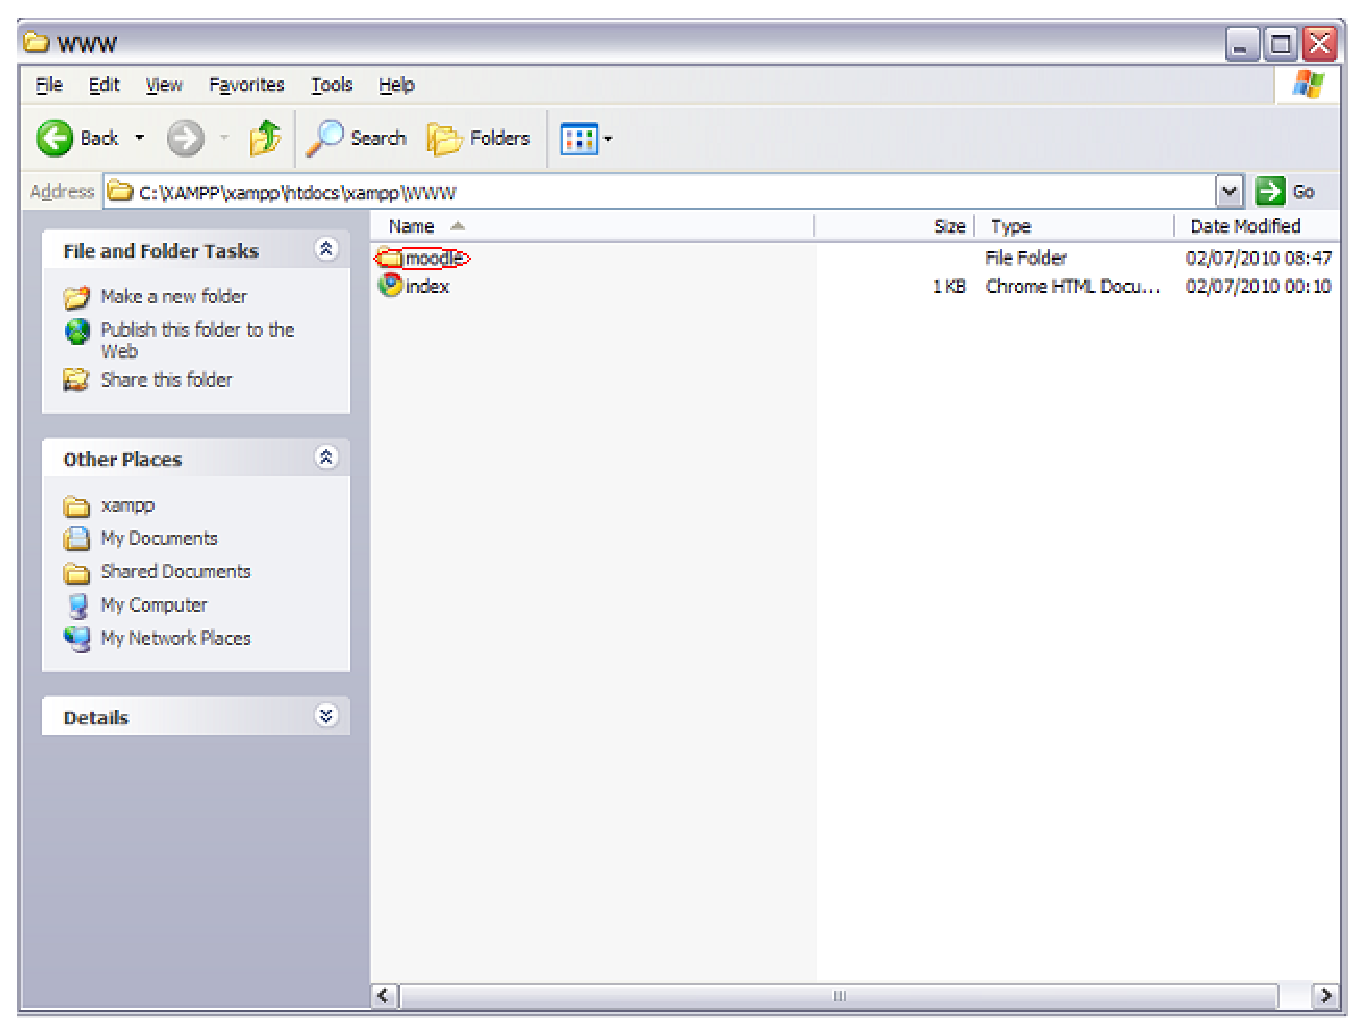
\includegraphics[width=1\textwidth]{char_narzarzedzi//rys//katalog_aplikacji.eps}
\end{figure}
Główny katalog Moodle'a w domyślnej konfiguracji ma nazwę \textit{moodle} \ref{rys:katalog_moodle} i znajdują się w nim podkatalogi i mając nawet nie wielką wiedzę na temat Moodle'a można szybko wywnioskować za co są odpowiedzialne. Na przykład katalog \textit{admin} przechowuje pliki PHP odpowiedzialne za generowanie strony administracyjne. Zaś katalog \textit{lang} przechowuje tłumaczenia interfejsu Moodle'a. Z kolei katalog \textit{mod} przechowuje różne moduły. \\
\begin{figure}[!h]
	\centering
		\caption{Katalog aplikacji Moodle'a} \label{rys:in_moodle}
\end{figure}
		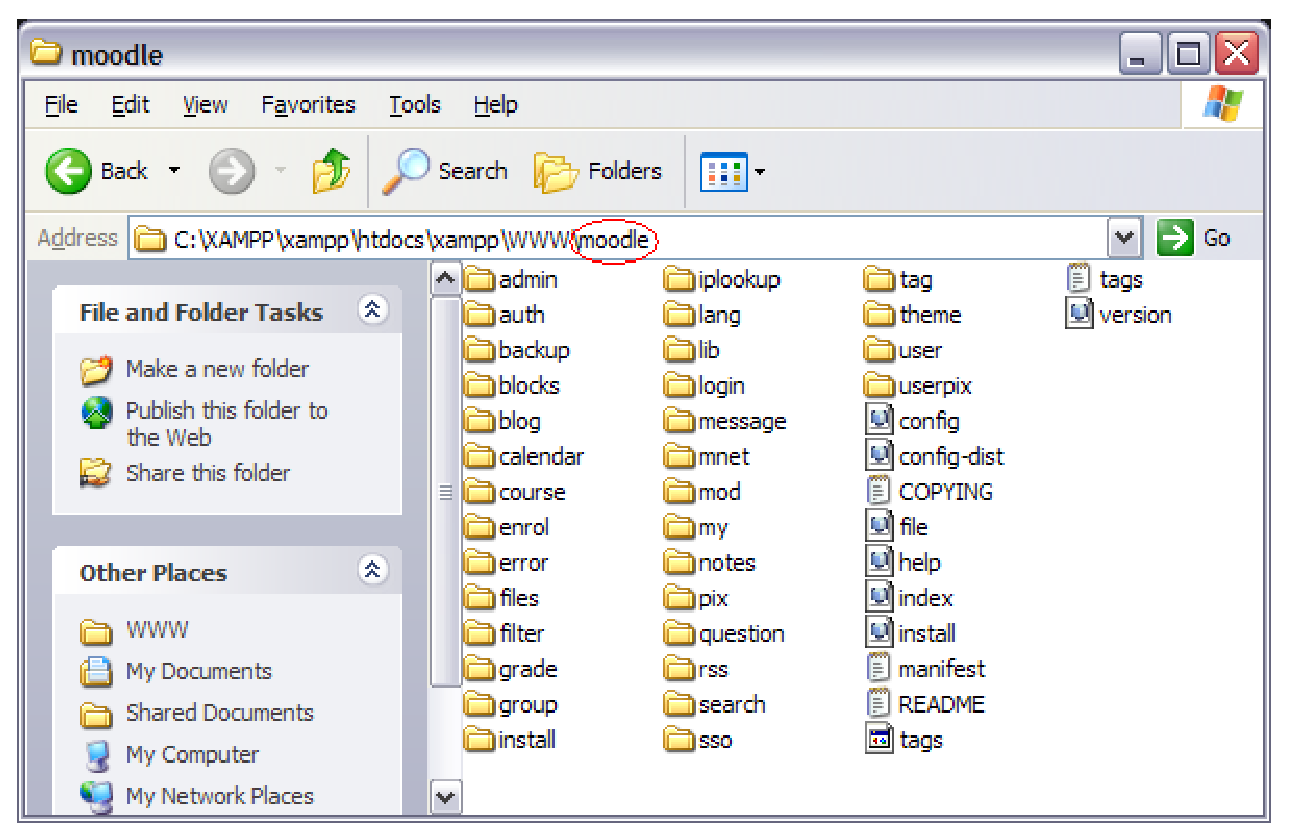
\includegraphics[width=1\textwidth]{char_narzarzedzi//rys//in_moodle.eps}
Rysunek \ref{rys:in_moodle} pokazuje całą zawartość głównego katalogu aplikacji. \\
Ponieważ każdy z podstawowych komponentów i modułów Moodle'a ma swój własny podkatalog. Dzięki temu mogą być one łatwo uaktualniane poprzez zamianę starych plików na nowymi. Dlatego warto sprawdzić co jakiś czas witrynę \href{http://www.moodle.org}{\textit{http://www.moodle.org}} w poszukiwaniu wiadomości o uaktualnieniach i poprawionych błędach. \\
\section{Katalog danych Moodle'a} \label{roz:moodledata}
\begin{figure}[!ht]
	\centering
		\caption{Katalog danych Moodle'a \textit{moodledata}} \label{rys:moodledata}
		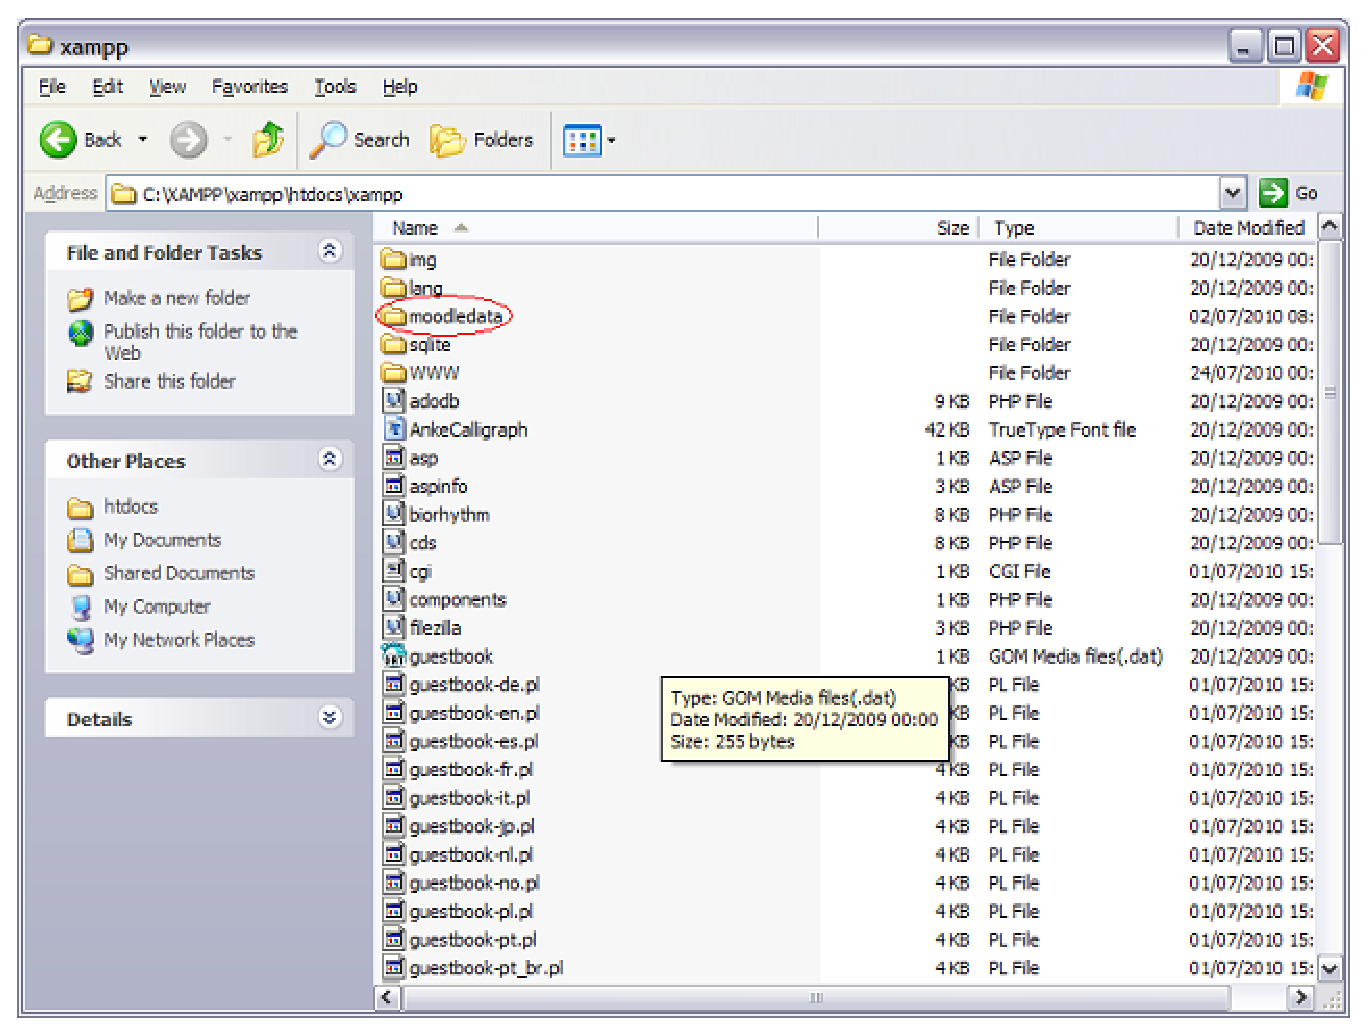
\includegraphics[width=1\textwidth]{char_narzarzedzi//rys//moodledata.eps}
\end{figure}
Wszystkie pliki przesyłane przez użytkowników są przechowywane w katalogu danych Moodle'a. Katalog ten podczas instalacji powinien być umieszczony tak aby nie było do niego dostępu z zewnątrz (internetu). To znaczy że nie powinno być możliwości dostania się do katalogu po wpisaniu jego adresu internetowego w przeglądarce. Są dwa sposoby zabezpieczenia tegoż katalogu. Pierwszy z nich dotyczy pliku \textit{.htaccess}. Zaś drugi, poprzez umieszczenie katalogu poza katalogiem dokumentów publicznych serwera. Jak pokazuje rysunek \ref{rys:moodledata}. Aby zabezpieczyć katalog przed przeglądaniem należy utworzyć w nim plik \textit{.htaccess} i wpisanie doń następujących komend:\\
\hspace{2cm} \texttt{order deny,allow} \\
\hspace{2cm} \texttt{deny from all} \\
\begin{figure}[!hb]
	\centering
		\caption{Wewnątrz katalogu \textit{moodledata}} \label{rys:in_moodledata}
		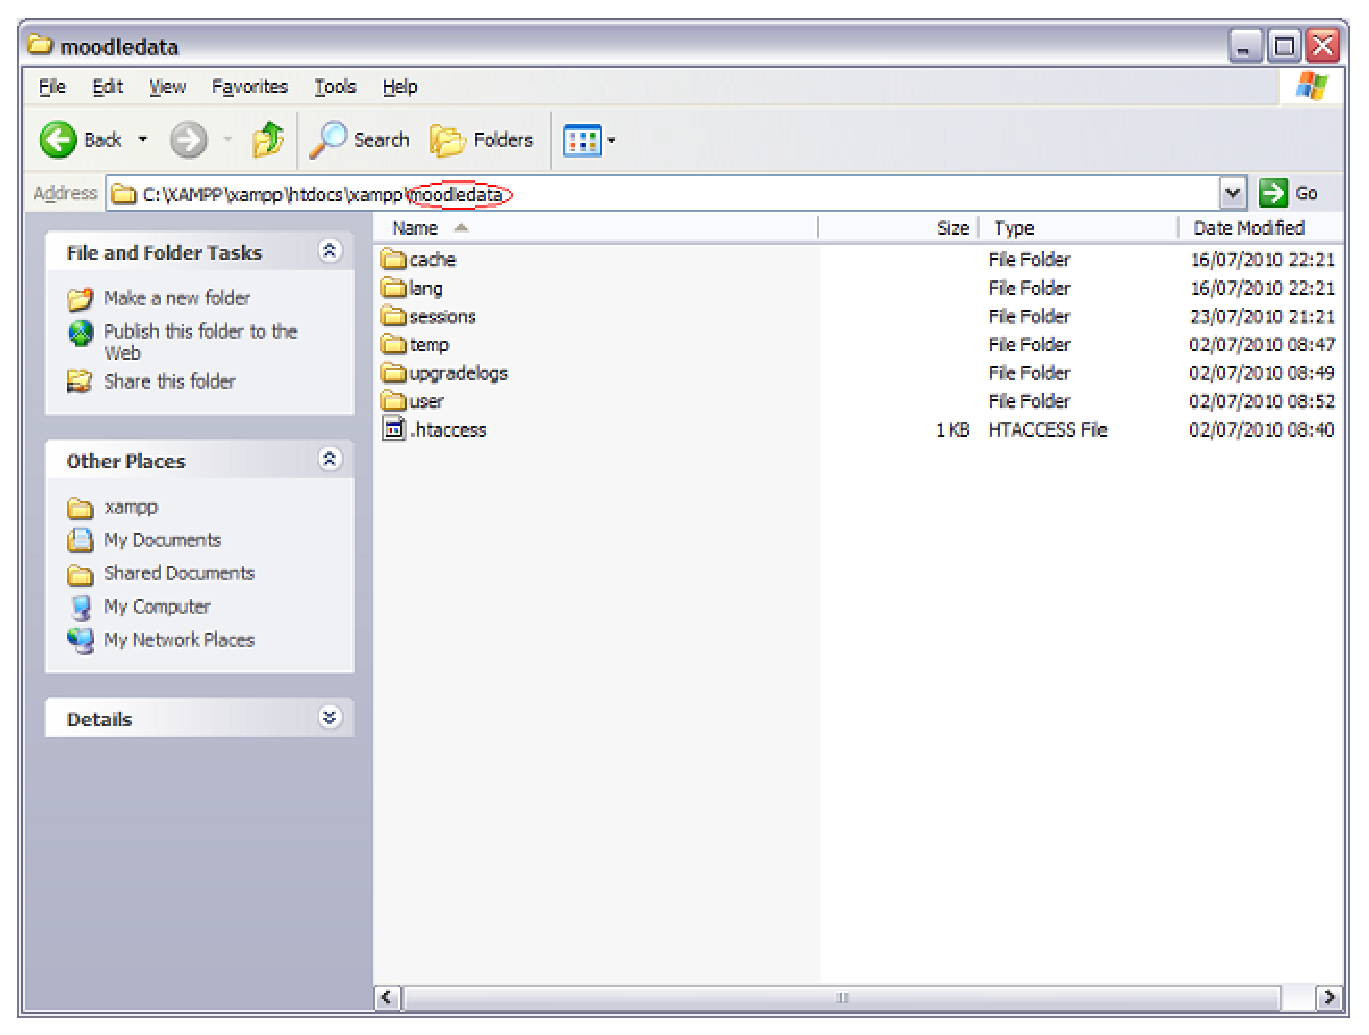
\includegraphics[width=1\textwidth]{char_narzarzedzi//rys//in_moodledata.eps}
\end{figure}
W przykładowej instalacji widać na rysunku\ref{rys:katalog_moodle} katalogiem dokumentów serwera jest \textit{$\backslash$WWW$\backslash$moodle}. Z tego powodu katalog danych został umieszczony poza katalogiem \textit{WWW} i katalogiem \textit{moodle}. Co widać na rysunku \ref{rys:moodledata}. Zaś rysunek \ref{rys:in_moodledata} pokazuje nam zawartość katalogu \textit{moodledata}. Jest tam również umieszczony plik \textit{.htaccess}. \\
\section{Baza danych Moodle'a} \label{roz:baza_dnaych}
\begin{figure}[!ht]
	\centering
		\caption{Kawałek bazy danych Moodle'a} \label{rys:baza}
		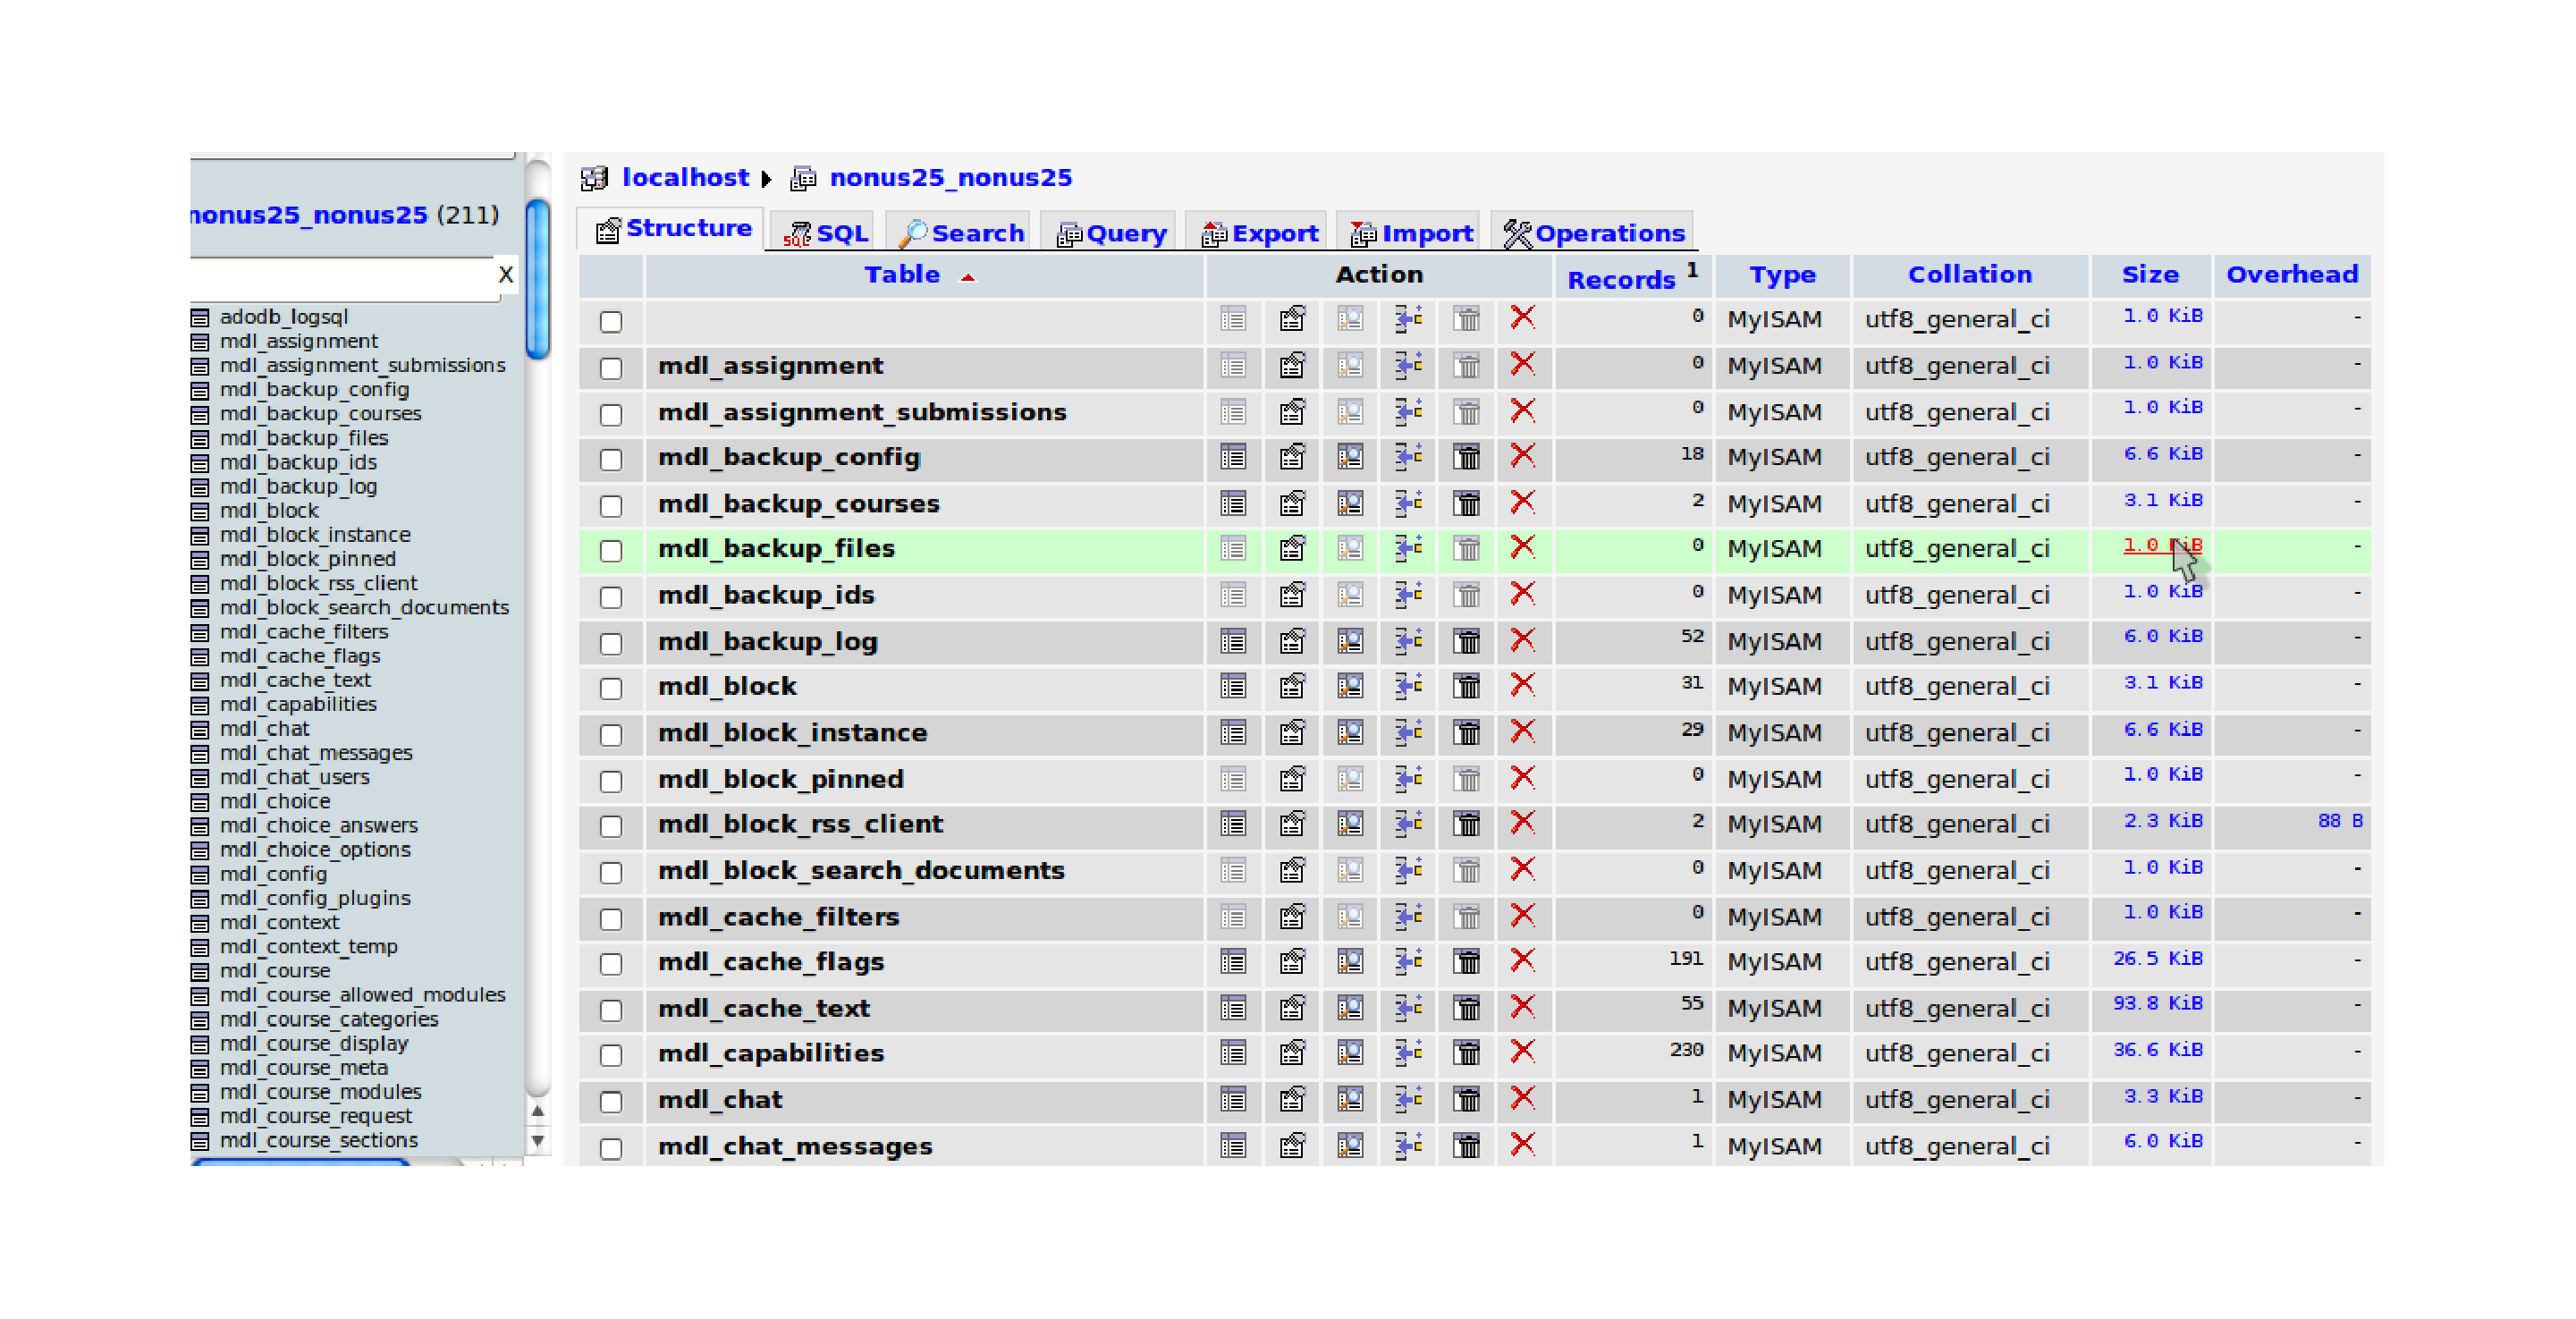
\includegraphics[width=1\textwidth]{char_narzarzedzi//rys//baza.eps}
\end{figure}
Podczas gdy katalog danych Moodle'a przechowuje pliki przesyłane przez użytkowników, bazy danych Moodle'a \ref{rys:baza} przechowują większość obiektów utworzonych za pomocą witryny Moodle'a, są przechowywane w postaci kodu HTML\footnote{HTML~-~język znaczników hipertekstu (ang. HyperText Markup Language} w bazie danych. Odnośniki dodawane do kursów, ustawienia i zawartość forów dyskusyjnych i stron wiki, quizy - wszystko to jest przykładem danych przechowywanych w bazie danych Moodle'a. Pokazuje to rysunek \ref{rys:tabela} \\
\begin{figure}[!hb]
	\centering
		\caption{Tabela \textit{mdl\_course}} \label{rys:tabela}
		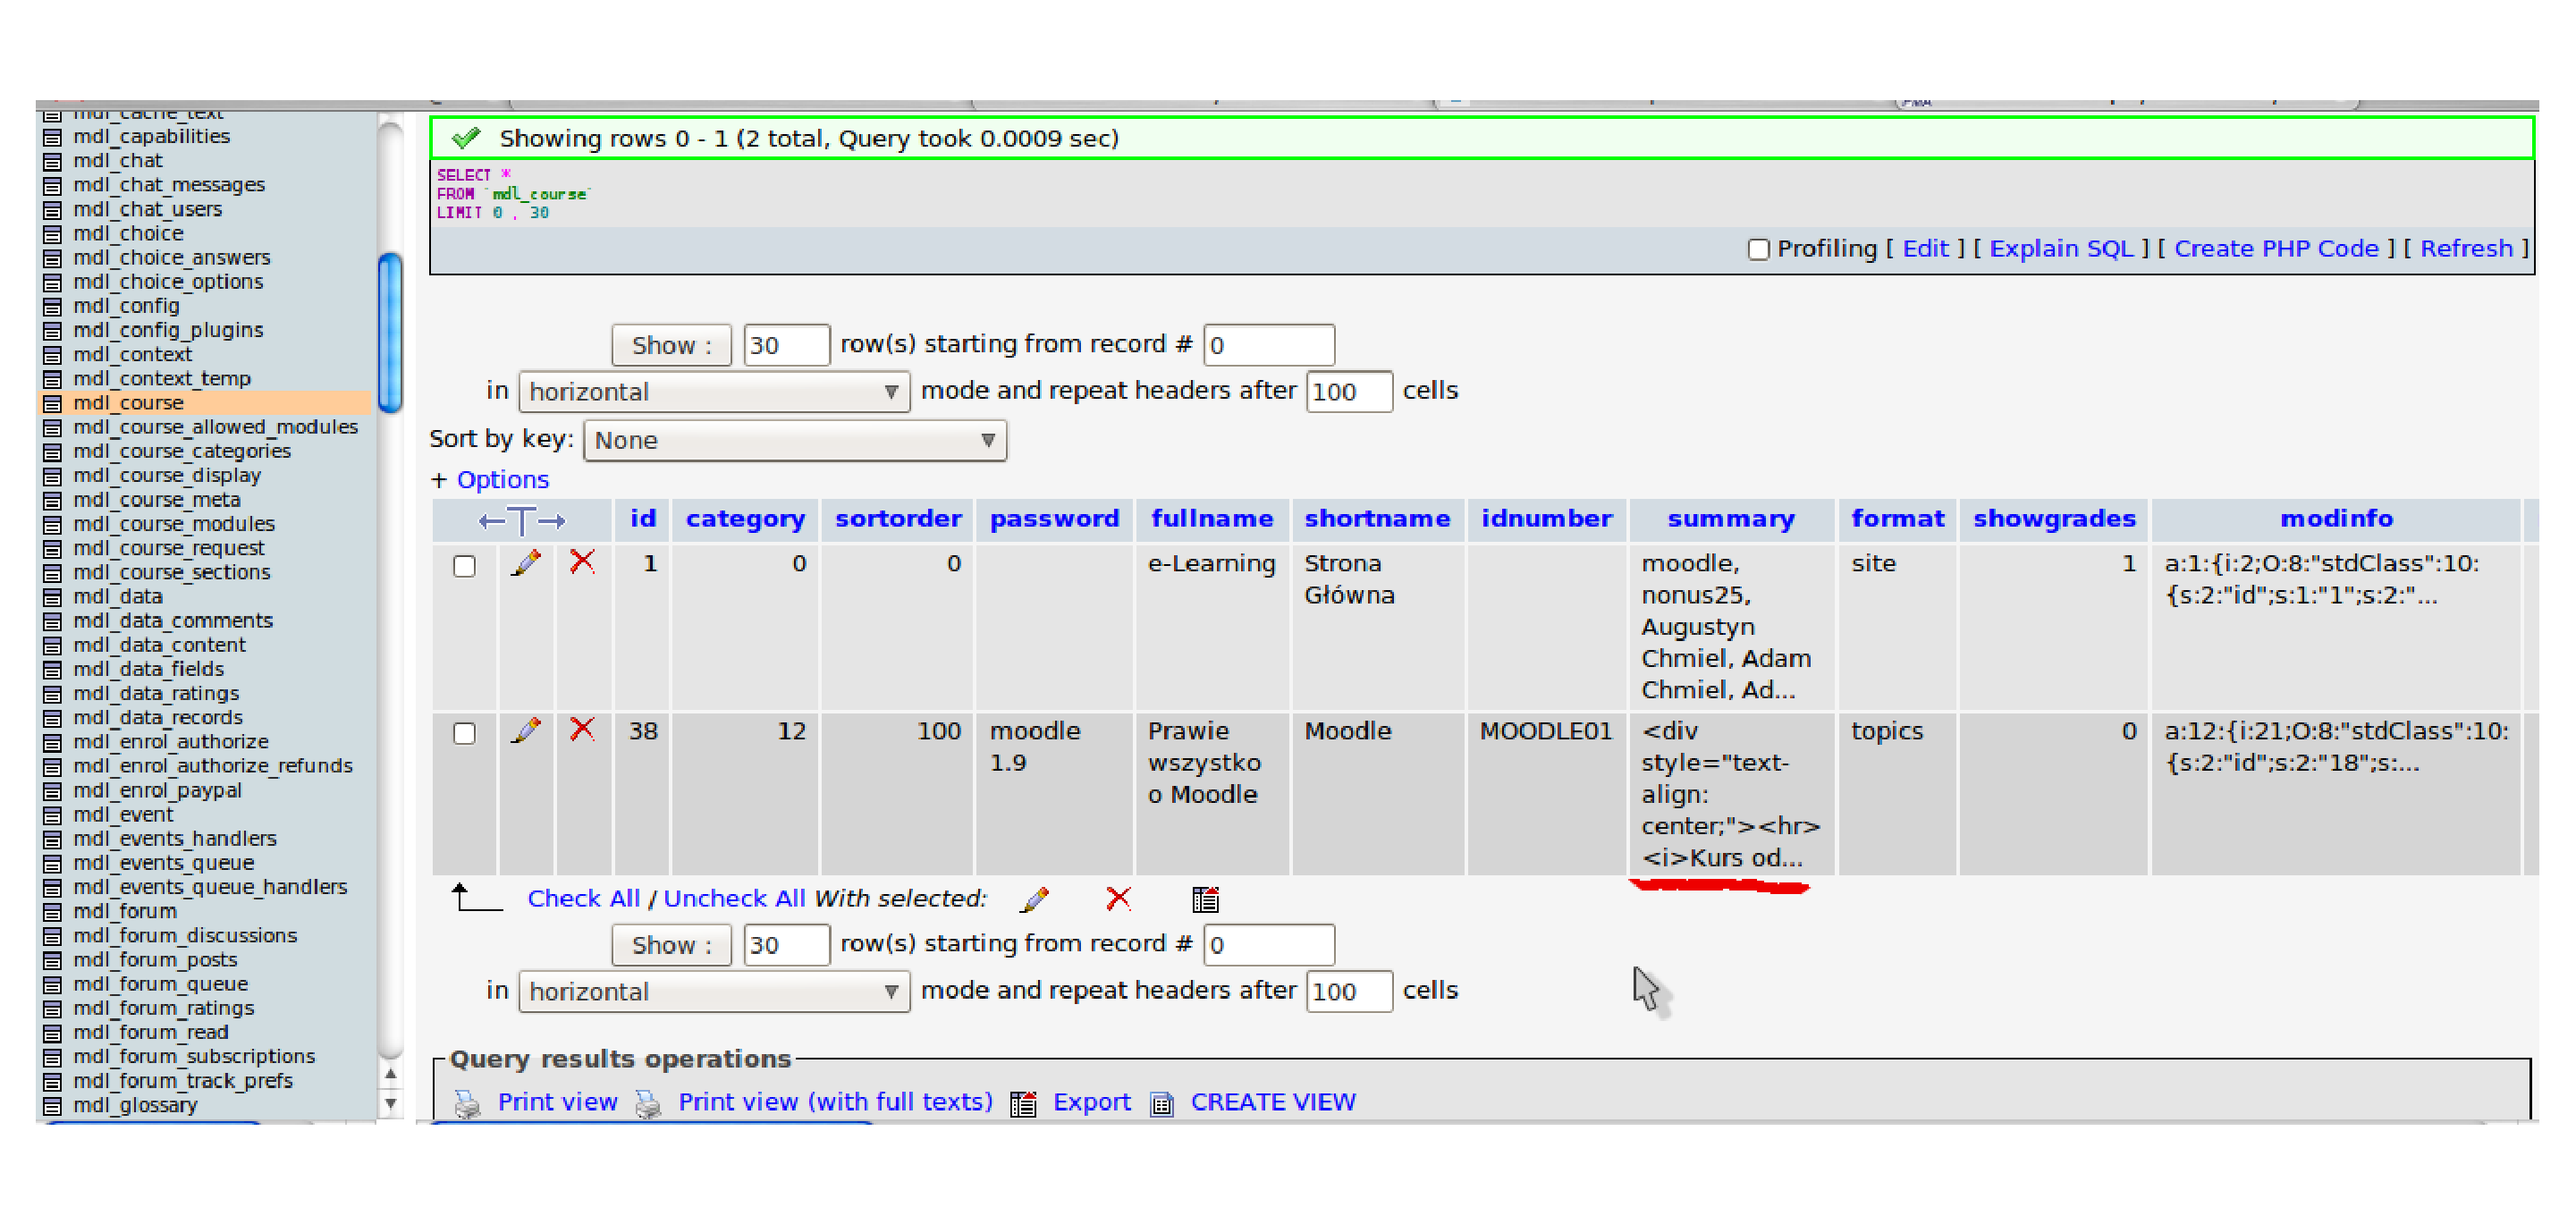
\includegraphics[width=1\textwidth]{char_narzarzedzi//rys//course.eps}
\end{figure}
Trzy części~-~\textbf{katalog aplikacji, katalog danych i baza danych}~-~współpracują ze sobą, tworząc witrynę nauczania. Interfejs w Moodle'u zachęca użytkownika do eksploracji i interakcji pomiędzy uczniami i nauczycielami oraz pomiędzy nimi samymi.\\
\section{Struktura katalogów \textit{Moodle'a}} \label{roz:struktura_moodle}
Aby lepiej zrozumieć strukture aplikacji Moodle'a wymienie i opisze podkatalogi zawarte w katalogu \textit{moodle}: \cite{dokumentacja_moodle}\\
	\begin{itemize}
		\item \textit{config.php}~-~zawiera podstawowe ustawienia. Ten plik nie jest częścią samego Moodle - zostanie utworzony podczas instalacji.
		\item \textit{install.php}~-~skrypt, który uruchomisz w celu utworzenia pliku \textit{config.php}. 
		\item \textit{version.php}~-~określa wersję kodu Moodle 
		\item \textit{index.php}~-~strona główna witryny
		\item \textit{admin/}~-~kod, służący do zarządzania serwerem
		\item \textit{auth/}~-~moduły wtyczek, służących do uwierzytelniania 
		\item \textit{blocks/}~-~moduły wtyczek, służących do obsługi małych bloków tekstowych, znajdujących się z boku wielu stron 
		\item \textit{calendar/}~-~kod, obsługujący zarządzanie i wyświetlanie kalendarzy 
		\item \textit{course/}~-~kod wyświetlający i zarządzający kursami 
		\item \textit{doc/}~-~dokumentacja pomocy Moodle
		\item \textit{files/}~-~kod wyświetlający i zarządzający plikami wysłanymi na serwer 
		\item \textit{lang/}~-~teksty w różnych językach, jeden katalog na język 
		\item \textit{lib/}~-~biblioteki rdzenia kodu Moodle 
		\item \textit{login/}~-~kod do obsługi kont 
		\item \textit{mod/}~-~zawiera wszystkie główne moduły kursów Moodle 
		\item \textit{pix/}~-~podstawowa grafika strony 
		\item \textit{theme/}~-~motywy graficzne/skórki, zmieniające wygląd strony 
		\item \textit{user/}~-~kod wyświetlający i zarządzający użytkownikami 
	\end{itemize}
